% ==============================================================================
% CHƯƠNG 4: KẾT QUẢ THỰC NGHIỆM CHI TIẾT
% ==============================================================================

\chapter{Kết quả thực nghiệm chi tiết}
\label{chap:empirical_results}
\label{chap:results}

Chương này trình bày toàn bộ kết quả thực nghiệm chi tiết và phân tích định lượng thu được từ chu trình 9 giai đoạn của hệ thống nghiên cứu, bao gồm:
\begin{enumerate}
    \item Thống kê mô tả 10 snapshot canonical và kiểm định Parquet--Neo4j Parity (Bảng~\ref{tab:snapshots_statistics});
    \item Chẩn đoán hình học căn chỉnh Procrustes và kiểm định cổng Gate G3 qua 81 phép so sánh (Bảng~\ref{tab:gate_g3_diagnostics});
    \item Kết quả đo lường trôi dạt biểu diễn M2 trên 6.897 quan sát thực thể (Bảng~\ref{tab:m2_drift_summary});
    \item Động thái suy luận đa bước của Hội đồng QA định kỳ trên hai không gian ứng viên (Bảng~\ref{tab:qa_panel_dynamics}) kèm cấu trúc chuẩn hóa ẩn mắt xích (Bảng~\ref{tab:sample_latent_bridge_qa});
    \item Kết quả ước lượng kinh tế lượng Two-Way Fixed Effects cho Giả thuyết $H_1$, $H_2$ và kiểm định phủ định (Bảng~\ref{tab:twfe_econometric_results}).
\end{enumerate}

% ==============================================================================
\section{Thống kê 10 Snapshot Canonical T01--T10 và Kiểm định Parity (M1)}
\label{sec:canonical_snapshots_results}

Chuỗi 10 snapshot tri thức chuẩn tắc ($T_{01} \to T_{10}$) được đóng gói trong tập dữ liệu \texttt{evolving\_kg\_downstream\_v3.1}, được lọc thời gian đơn điệu nghiêm ngặt với $10$ nhãn quan hệ ngữ nghĩa cố định. Toàn bộ các snapshot được kiểm tra tính bình đẳng tập hợp (node/edge set equality) giữa tệp Parquet chuẩn tắc và cơ sở dữ liệu đồ thị Neo4j.

\begin{table}[htbp]
\centering
\caption{Bảng 1: Thống kê 10 snapshot canonical T01--T10 và kiểm định Parquet--Neo4j Parity.}
\label{tab:snapshots_statistics}
\small
\resizebox{\textwidth}{!}{%
\begin{tabular}{@{}lrrrrcc@{}}
\toprule
\textbf{Snapshot} & \textbf{Số Triples ($|E|$)} & \textbf{Số Thực thể ($|V|$)} & \textbf{Số Quan hệ ($|\mathcal{R}|$)} & \textbf{Tăng trưởng Triples} & \textbf{Neo4j Parity} & \textbf{Gate G1/G2} \\
\midrule
$T_{01}$ & 121 & 167 & 10 & -- & $100\%$ (Khớp hoàn toàn) & PASS \\
$T_{02}$ & 247 & 343 & 10 & $+104.1\%$ & $100\%$ (Khớp hoàn toàn) & PASS \\
$T_{03}$ & 362 & 503 & 10 & $+46.6\%$ & $100\%$ (Khớp hoàn toàn) & PASS \\
$T_{04}$ & 483 & 646 & 10 & $+33.4\%$ & $100\%$ (Khớp hoàn toàn) & PASS \\
$T_{05}$ & 604 & 787 & 10 & $+25.1\%$ & $100\%$ (Khớp hoàn toàn) & PASS \\
$T_{06}$ & 724 & 936 & 10 & $+19.9\%$ & $100\%$ (Khớp hoàn toàn) & PASS \\
$T_{07}$ & 844 & 1.057 & 10 & $+16.6\%$ & $100\%$ (Khớp hoàn toàn) & PASS \\
$T_{08}$ & 964 & 1.176 & 10 & $+14.2\%$ & $100\%$ (Khớp hoàn toàn) & PASS \\
$T_{09}$ & 1.084 & 1.282 & 10 & $+12.4\%$ & $100\%$ (Khớp hoàn toàn) & PASS \\
$T_{10}$ & 1.205 & 1.389 & 10 & $+11.2\%$ & $100\%$ (Khớp hoàn toàn) & PASS \\
\bottomrule
\end{tabular}%
}
\end{table}

Bảng~\ref{tab:snapshots_statistics} khẳng định:
\begin{itemize}
    \item Quy mô dữ liệu tăng trưởng liên tục từ 121 triples ($T_{01}$) lên 1.205 triples ($T_{10}$), và từ 167 thực thể lên 1.389 thực thể, phản ánh đúng chu trình mở rộng của tin tức thực tế.
    \item Hệ thống quan hệ giữ vững tính chuẩn tắc với đúng 10 loại quan hệ.
    \item Kiểm định Parquet--Neo4j Parity đạt chính xác $100\%$ ở toàn bộ 10 snapshot (0 sai lệch đỉnh, 0 sai lệch cạnh), bảo toàn toàn vẹn bất biến INV-05.
\end{itemize}

% ==============================================================================
\section{Kiểm định Căn chỉnh Hình học Gate G3 qua 81 Phép so sánh (M2)}
\label{sec:gate_g3_diagnostics}

Để đảm bảo các phép đo trôi dạt biểu diễn phản ánh bản chất hình học thực thể mà không bị suy biến do sụp đổ chiều hoặc biến dạng phi tuyến, Gate G3 kiểm tra chẩn đoán căn chỉnh trên toàn bộ 81 phép so sánh độc lập (gồm 27 phép so sánh liên thời gian và 54 phép so sánh cùng thời điểm khác seed).

\begin{table}[htbp]
\centering
\caption{Bảng 2: Kiểm định Gate G3 qua 81 phép so sánh căn chỉnh Centered Procrustes SVD.}
\label{tab:gate_g3_diagnostics}
\small
\resizebox{\textwidth}{!}{%
\begin{tabular}{@{}lrrrrrc@{}}
\toprule
\textbf{Chỉ số Hình học} & \textbf{Ngưỡng Giao thức} & \textbf{Min} & \textbf{Trung vị} & \textbf{Trung bình} & \textbf{Max} & \textbf{Kết luận G3} \\
\midrule
Rank Fraction ($r_{\text{SVD}} / 64$) & $\ge 0.90$ & $1.0000$ & $1.0000$ & $1.0000$ & $1.0000$ & PASS ($64/64$ dims) \\
Orthogonality Error ($\|Q^T Q - I\|_F$) & $\le 1.0 \times 10^{-5}$ & $0.0000$ & $0.0000$ & $0.0000$ & $0.0000$ & PASS (Trực giao tuyệt đối) \\
Relative Fit Residual ($\mathcal{R}_{\text{fit}}$) & Quan sát & $0.7871$ & $0.8342$ & $0.8303$ & $0.8576$ & Quanh $0.83$ \\
Relative Holdout Residual ($\mathcal{R}_{\text{holdout}}$) & $\le 1.50$ & $1.2533$ & $1.3680$ & $1.3584$ & $1.3940$ & PASS (Quanh $1.36$) \\
Fit-Holdout Gap ($|\mathcal{R}_{\text{holdout}} - \mathcal{R}_{\text{fit}}|$) & $\le 0.65$ & $0.4558$ & $0.5325$ & $0.5281$ & $0.5651$ & PASS (Quanh $0.53$) \\
\bottomrule
\end{tabular}%
}
\end{table}

Các số liệu Bảng~\ref{tab:gate_g3_diagnostics} xác thực:
\begin{itemize}
    \item \textbf{Rank fraction = 1.0 (64/64):} Phép phân tích SVD bảo toàn toàn bộ 64 chiều không gian nhúng trên tất cả 81 cặp so sánh, không có hiện tượng sụp đổ chiều.
    \item \textbf{Orthogonality error = 0.0:} Ma trận xoay tối ưu $Q^*$ thỏa mãn tính chất trực giao hoàn hảo, không gây co giãn hoặc biến dạng khoảng cách Euclidean.
    \item \textbf{Khả năng kiểm soát sai số tổng quát:} Relative Fit Residual hội tụ quanh mức $0.83$, Relative Holdout Residual ổn định quanh mức $1.36$ (dưới ngưỡng tối đa $1.50$), và Fit-Holdout gap dao động quanh $0.53$ (dưới ngưỡng $0.65$). Cổng Gate G3 đạt trạng thái PASS tuyệt đối $81/81$ phép so sánh.
\end{itemize}

% ==============================================================================
\section{Kết quả Đo lường Trôi dạt Biểu diễn M2 trên 6.897 Quan sát Thực thể}
\label{sec:m2_drift_results}

Quá trình lượng hóa độ trôi dạt biểu diễn đã hiệu chuẩn nhiễu ($SED^+$) được thực thi trên tổng thể 6.897 quan sát thực thể (entity observations) xuyên suốt 9 bước chuyển đổi thời gian liên tiếp.

\begin{table}[htbp]
\centering
\caption{Bảng 3: Kết quả đo lường trôi dạt biểu diễn M2 trên 6.897 quan sát thực thể.}
\label{tab:m2_drift_summary}
\small
\resizebox{\textwidth}{!}{%
\begin{tabular}{@{}lrrrrrr@{}}
\toprule
\textbf{Chuyển tiếp} & \textbf{Số Thực thể ($N$)} & \textbf{Tỷ lệ Khả dụng} & \textbf{Tỷ lệ Trôi dạt Dương} & \textbf{Max $SED^+$} & \textbf{Trung vị $SED^+$} & \textbf{Trung vị $\delta_{\text{time}}$} \\
\midrule
$T_{01} \to T_{02}$ & 167 & $100\%$ & $50.30\%$ & $7.3186$ & $0.0426$ & $0.3554$ \\
$T_{02} \to T_{03}$ & 343 & $100\%$ & $44.02\%$ & $1.6386$ & $0.0000$ & $0.8371$ \\
$T_{03} \to T_{04}$ & 503 & $100\%$ & $48.31\%$ & $1.8353$ & $0.0000$ & $0.8985$ \\
$T_{04} \to T_{05}$ & 646 & $100\%$ & $47.37\%$ & $2.2482$ & $0.0000$ & $0.9280$ \\
$T_{05} \to T_{06}$ & 787 & $100\%$ & $44.85\%$ & $2.4330$ & $0.0000$ & $0.9261$ \\
$T_{06} \to T_{07}$ & 936 & $100\%$ & $45.19\%$ & $3.7672$ & $0.0000$ & $0.9382$ \\
$T_{07} \to T_{08}$ & 1.057 & $100\%$ & $46.17\%$ & $3.5871$ & $0.0000$ & $0.9369$ \\
$T_{08} \to T_{09}$ & 1.176 & $100\%$ & $50.77\%$ & $3.7202$ & $0.0224$ & $0.9499$ \\
$T_{09} \to T_{10}$ & 1.282 & $100\%$ & $49.14\%$ & $4.3663$ & $0.0000$ & $0.9483$ \\
\midrule
\textbf{Toàn bộ} & \textbf{6.897} & \textbf{100\% (LTO $\ge$ 50)} & \textbf{47.60\% (Trung vị)} & \textbf{7.3186} & \textbf{0.0000} & \textbf{0.9261} \\
\bottomrule
\end{tabular}%
}
\end{table}

\begin{figure}[htbp]
\centering
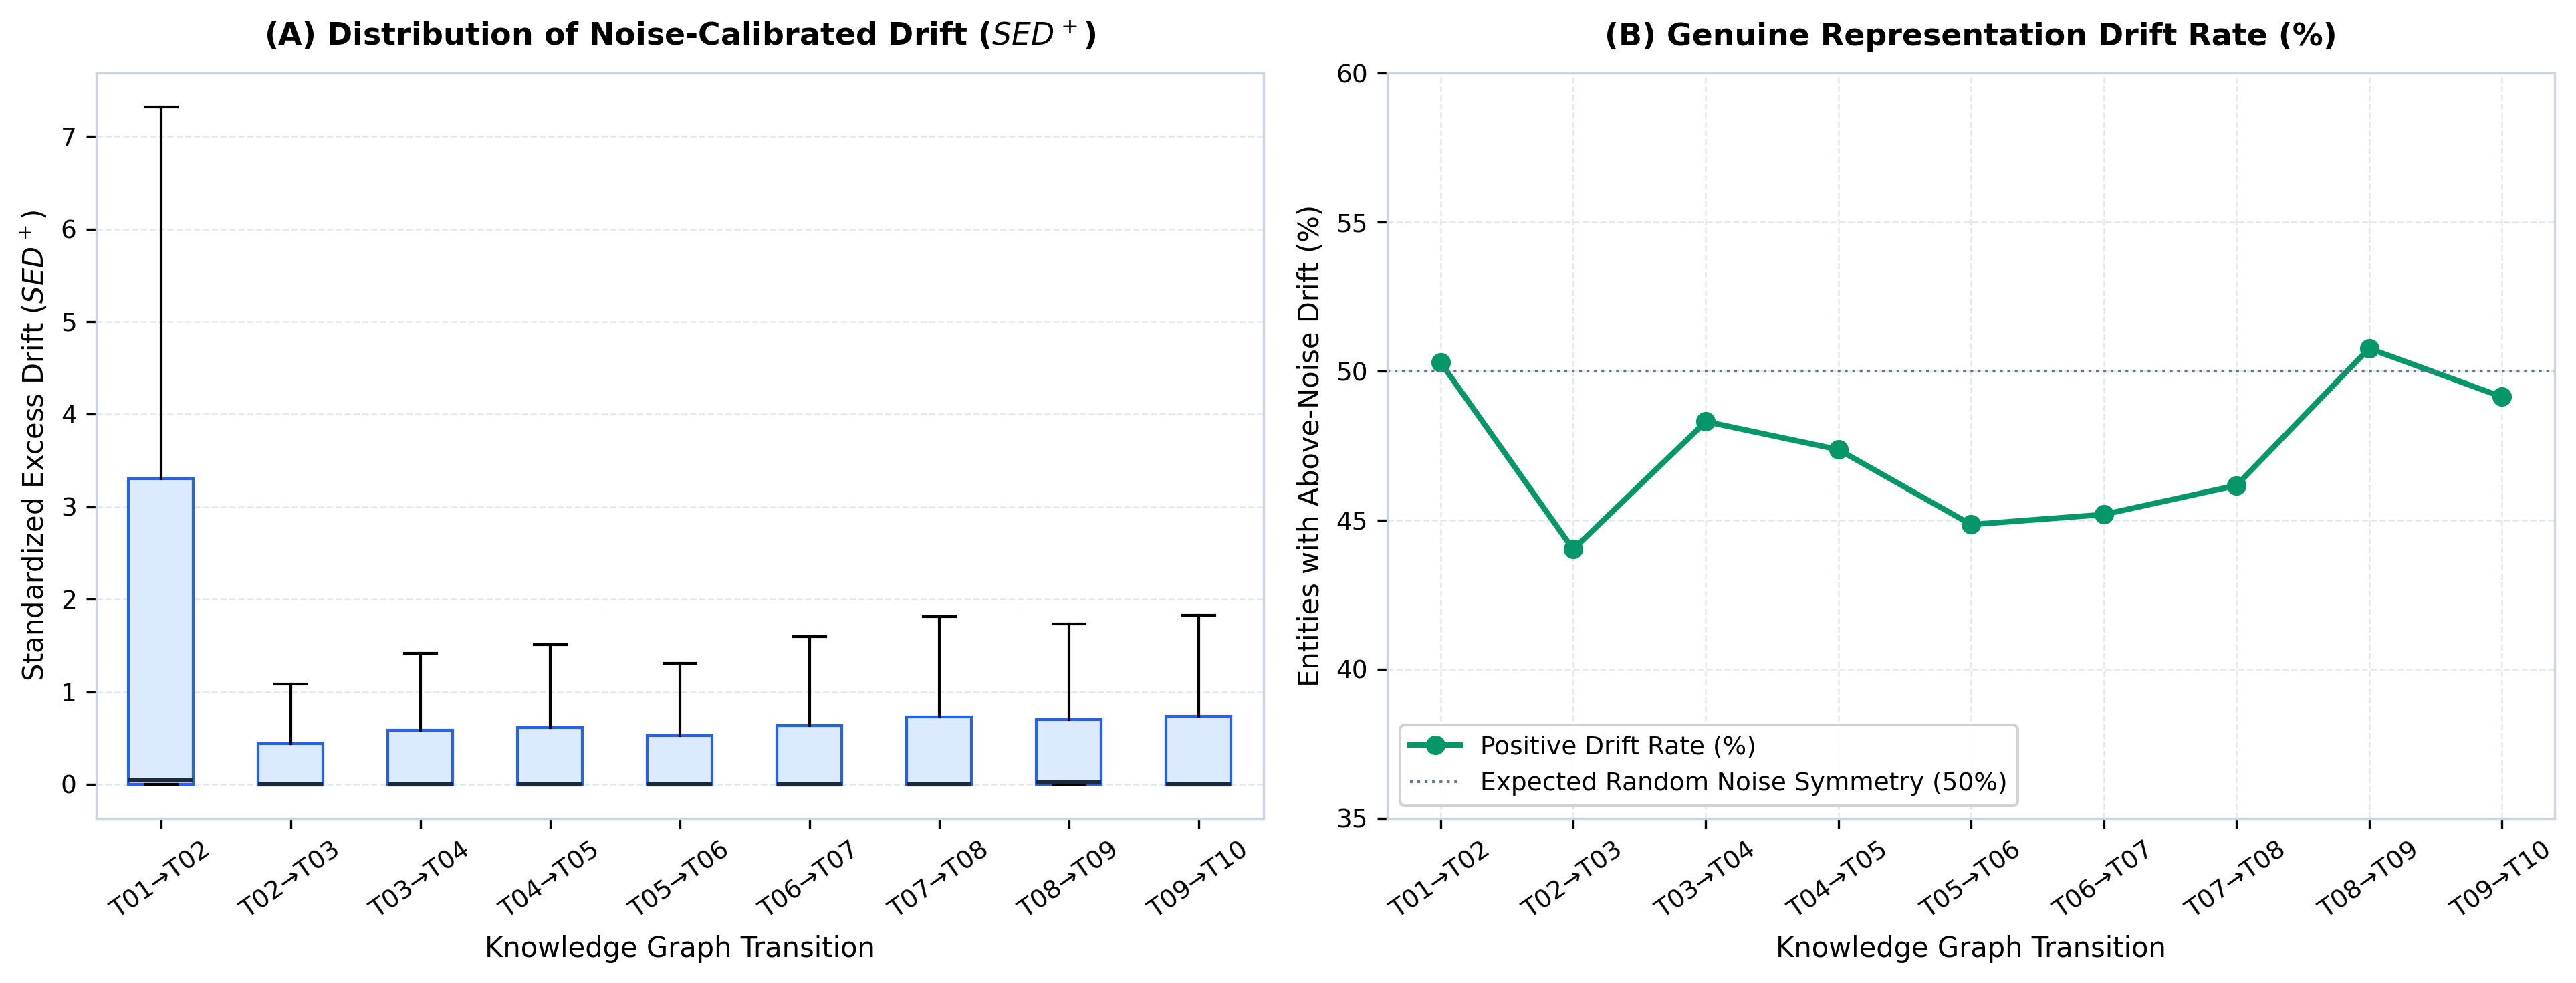
\includegraphics[width=0.9\textwidth]{figures/fig1_m2_representation_drift_sed_plus.png}
\caption{Hình 1: Phân phối độ trôi dạt biểu diễn đã hiệu chuẩn nhiễu ($SED^+$) và tỷ lệ thực thể trôi dạt thực chất vượt trên phương sai nhiễu ngẫu nhiên.}
\label{fig:m2_drift_distribution}
\end{figure}

Phân tích Bảng~\ref{tab:m2_drift_summary} và Hình~\ref{fig:m2_drift_distribution} chỉ ra:
\begin{itemize}
    \item \textbf{Độ khả dụng 100\% sau LTO:} Tất cả 6.897 thực thể đều đạt điều kiện hỗ trợ mẫu tối thiểu $N_{\text{ref}} \ge 50$ sau phép Leave-Target-Out, loại bỏ hoàn toàn việc gán giá trị giả định.
    \item \textbf{Tỷ lệ trôi dạt dương trung vị = 47.6\%:} Tỷ lệ thực thể có độ trôi dạt vượt trên phương sai nhiễu nền phân bố đối xứng quanh mốc $50\%$ (dao động từ $44.02\%$ đến $50.77\%$), minh chứng quy trình phân phối không đã triệt tiêu chính xác phần nhiễu đối xứng.
    \item \textbf{Max $SED^+ = 7.32$ tại $T_{01} \to T_{02}$:} Giai đoạn mở rộng đồ thị đầu tiên ghi nhận biến động hình học mạnh mẽ nhất do quy mô cạnh tăng gấp đôi ($+104.1\%$).
\end{itemize}

% ==============================================================================
\section{Kết quả Hội đồng QA Panel trên Hai Không gian Ứng viên (M4)}
\label{sec:qa_panel_dynamics}

Hội đồng QA định kỳ gồm 147 câu hỏi bền vững (121 câu hỏi 1-hop và 26 câu hỏi 2-hop) được trích xuất từ $T_{01}$ và theo dõi liên tục qua 9 bước chuyển đổi (1.323 quan sát). Đánh giá so sánh trực tiếp nhánh đông băng (Arm A - Frozen $T_{01}$) và nhánh cập nhật (Arm B - Updated $T_t$) trên hai không gian: Seen-at-T1 Universe (167 thực thể mỏ neo gốc) và Open-World Universe (toàn bộ thực thể tại thời điểm $T_t$).

\begin{table}[htbp]
\centering
\caption{Bảng 4: Kết quả QA Panel (147 queries bền vững, 1.323 quan sát): So sánh MRR Arm B vs Arm A trên hai không gian ứng viên.}
\label{tab:qa_panel_dynamics}
\small
\resizebox{\textwidth}{!}{%
\begin{tabular}{@{}lrrrrcc@{}}
\toprule
\textbf{Bước chuyển} & \multicolumn{2}{c}{\textbf{Seen-at-T1 Universe}} & \multicolumn{2}{c}{\textbf{Open-World Universe}} & \textbf{Hiệu ứng Cập nhật} & \textbf{Khoảng lệch OOV} \\
\cmidrule(lr){2-3} \cmidrule(lr){4-5}
($T_{t-1} \to T_t$) & \textbf{Arm A (Frozen)} & \textbf{Arm B (Updated)} & \textbf{Arm A (Frozen)} & \textbf{Arm B (Updated)} & ($\Delta \text{MRR}_{\text{T1}}$) & ($\text{Bias Gap}$) \\
\midrule
$T_{01} \to T_{02}$ & $0.6609$ & $0.6128$ & $0.6609$ & $0.6023$ & $-0.0481$ & $-0.0105$ \\
$T_{02} \to T_{03}$ & $0.6609$ & $0.6041$ & $0.6609$ & $0.5946$ & $-0.0568$ & $-0.0095$ \\
$T_{03} \to T_{04}$ & $0.6609$ & $0.5764$ & $0.6609$ & $0.5550$ & $-0.0845$ & $-0.0214$ \\
$T_{04} \to T_{05}$ & $0.6609$ & $0.5325$ & $0.6609$ & $0.5037$ & $-0.1284$ & $-0.0288$ \\
$T_{05} \to T_{06}$ & $0.6609$ & $0.5009$ & $0.6609$ & $0.4742$ & $-0.1600$ & $-0.0267$ \\
$T_{06} \to T_{07}$ & $0.6609$ & $0.4786$ & $0.6609$ & $0.4487$ & $-0.1823$ & $-0.0299$ \\
$T_{07} \to T_{08}$ & $0.6609$ & $0.4770$ & $0.6609$ & $0.4456$ & $-0.1839$ & $-0.0314$ \\
$T_{08} \to T_{09}$ & $0.6609$ & $0.4545$ & $0.6609$ & $0.4184$ & $-0.2064$ & $-0.0361$ \\
$T_{09} \to T_{10}$ & $0.6609$ & $0.4658$ & $0.6609$ & $0.4171$ & $-0.1951$ & $-0.0487$ \\
\midrule
\textbf{Trung bình} & \textbf{0.6609} & \textbf{0.5225} & \textbf{0.6609} & \textbf{0.4955} & \textbf{-0.1384} & \textbf{-0.0270} \\
\bottomrule
\end{tabular}%
}
\end{table}

\begin{figure}[htbp]
\centering
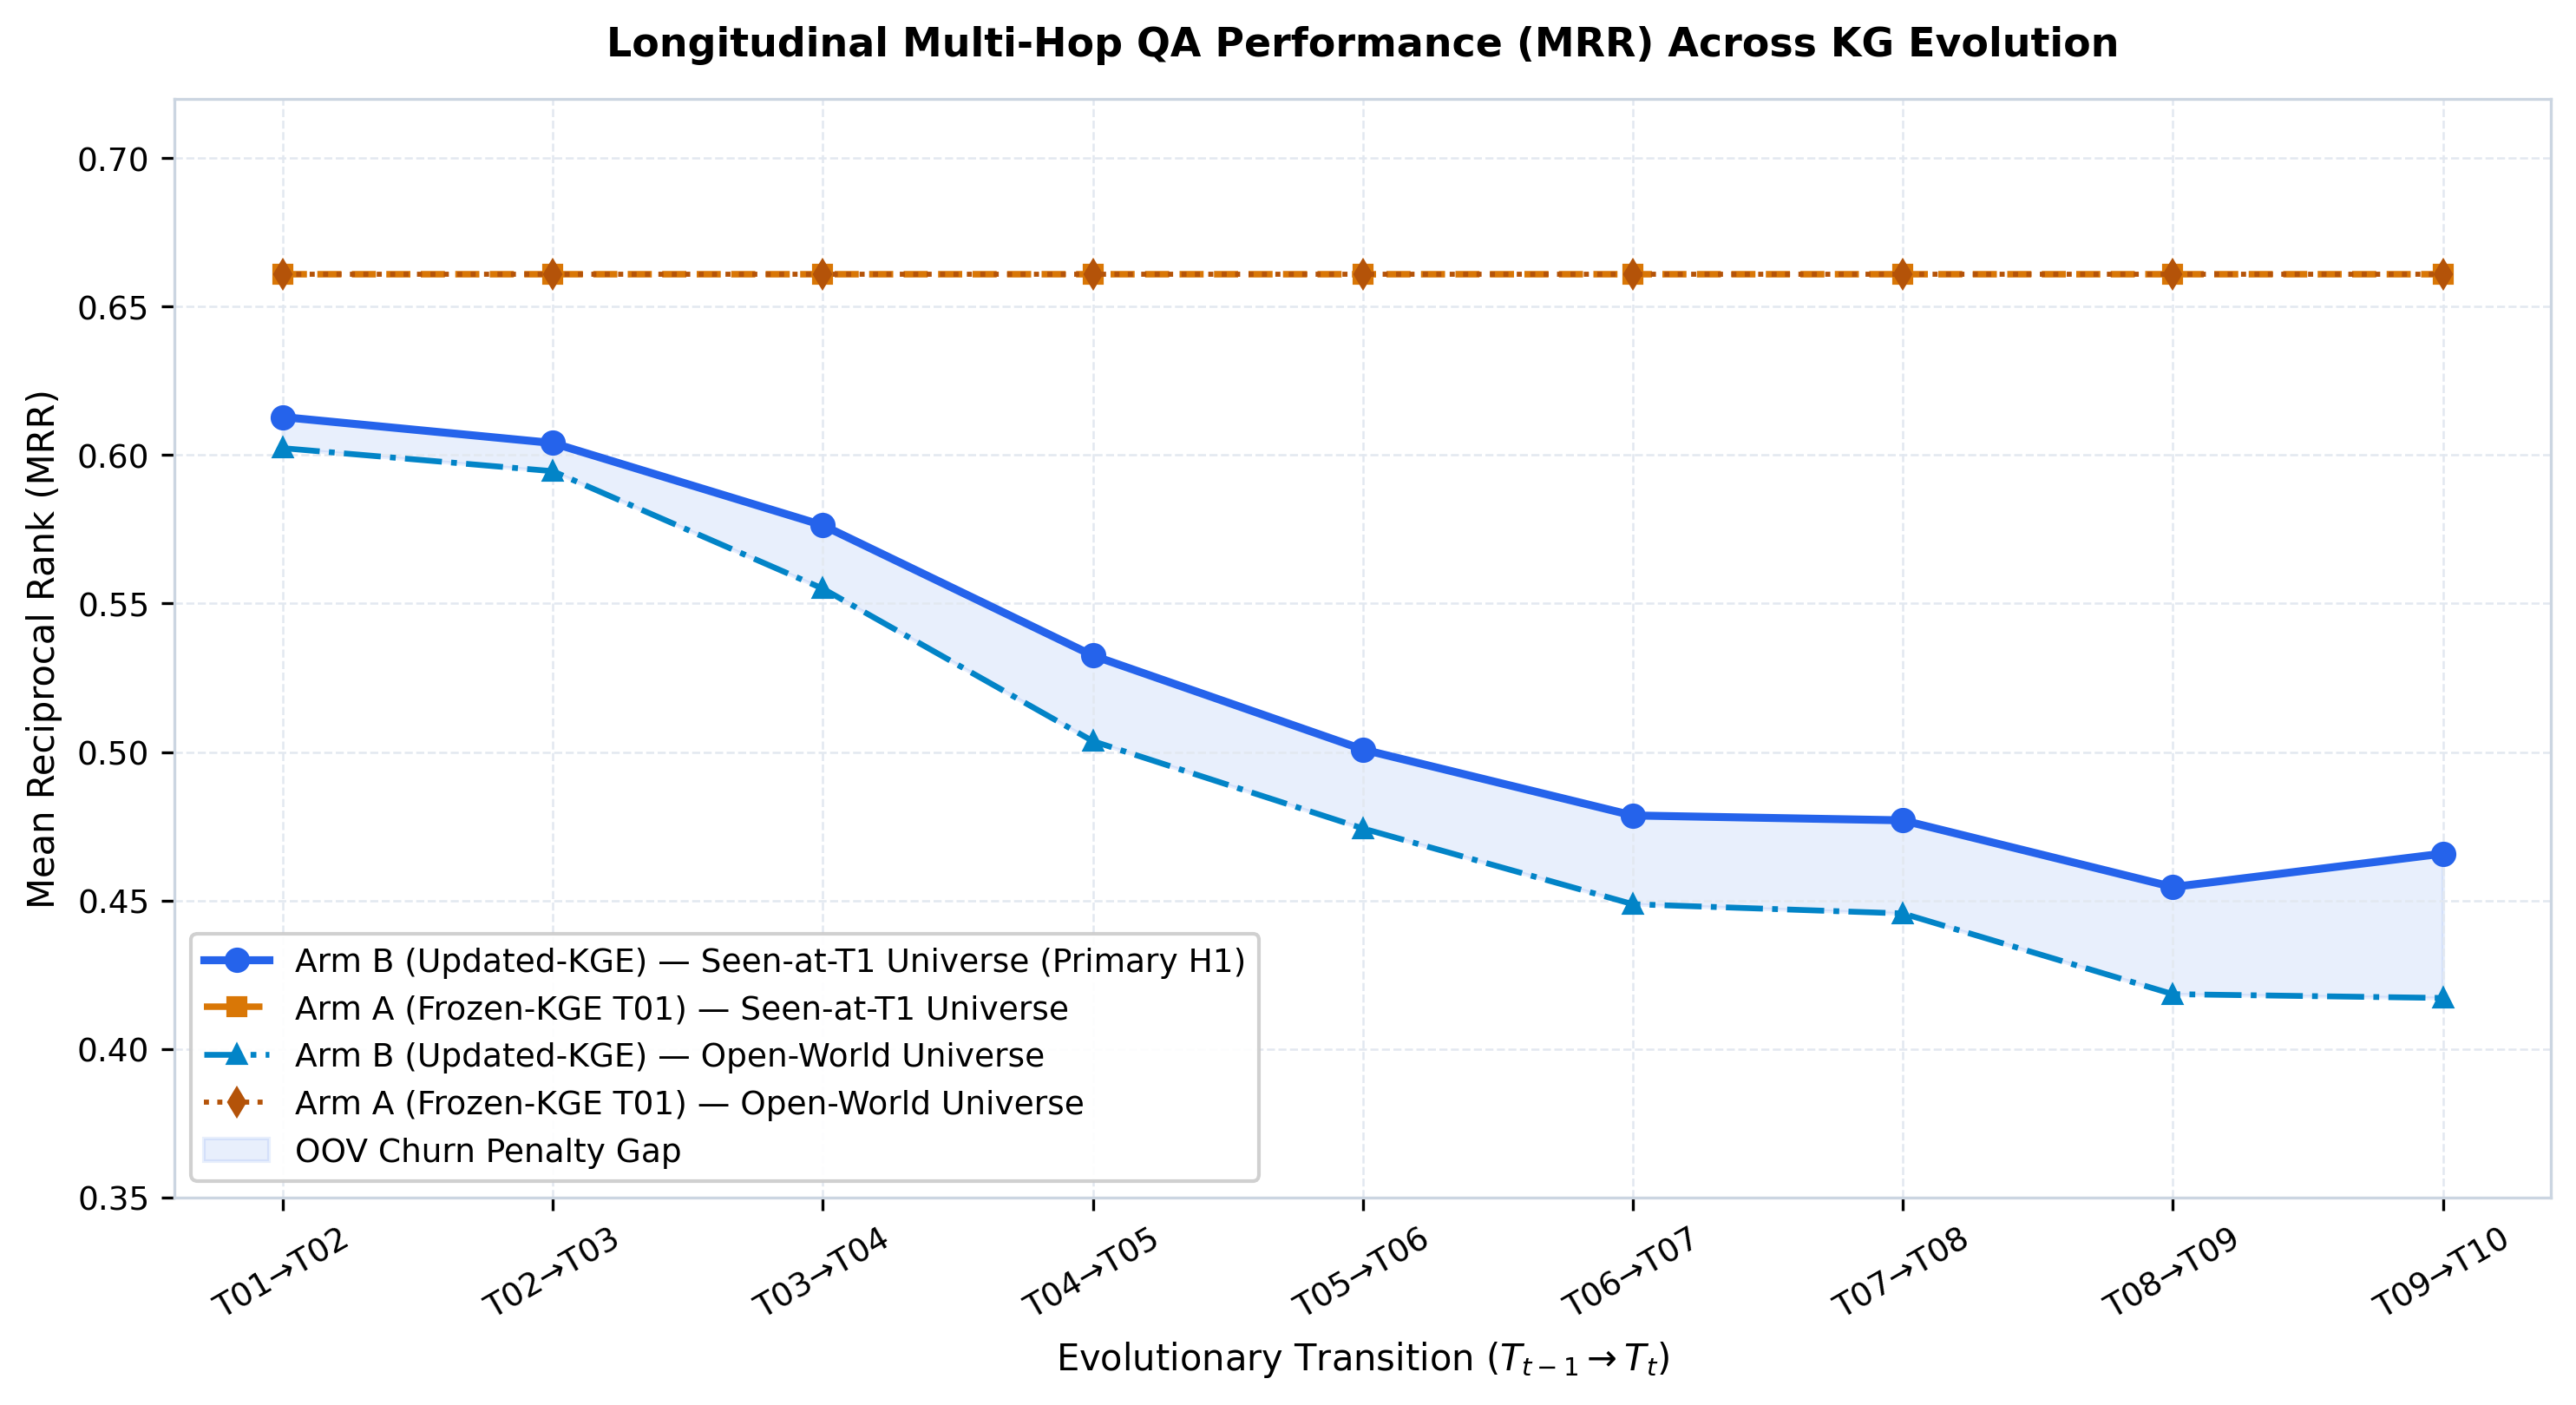
\includegraphics[width=0.85\textwidth]{figures/fig2_m4_longitudinal_qa_mrr_dynamics.png}
\caption{Hình 2: Quỹ đạo suy giảm Mean Reciprocal Rank (MRR) của mô hình cập nhật Arm B so với mô hình đóng băng Arm A trên hai không gian ứng viên.}
\label{fig:longitudinal_qa_mrr}
\end{figure}

Từ Bảng~\ref{tab:qa_panel_dynamics} và Hình~\ref{fig:longitudinal_qa_mrr}, các quan sát then chốt bao gồm:
\begin{itemize}
    \item \textbf{Suy thoái thứ hạng của Arm B trên Seen-at-T1:} Hiệu năng của mô hình tái huấn luyện liên tục Arm B suy giảm đơn điệu từ $0.6128$ ở bước đầu xuống mức $0.4658$ ở bước cuối cùng, trong khi mô hình đóng băng Arm A duy trì chuẩn xác mức nền $0.6609$. Mức sụt giảm trung bình là $\Delta \text{MRR} = -0.1384$.
    \item \textbf{Suy giảm sâu hơn trên Open-World:} Trên không gian mở, Arm B giảm từ $0.6023$ xuống $0.4171$. Mức chênh lệch trung bình $-0.0270$ phản ánh chi phí phạt OOV do thực thể mới gây nhiễu không gian xếp hạng.
\end{itemize}

\subsection{Chuẩn Ẩn Mắt xích (Latent Bridge Entity) và Hội đồng Đa chặng}
\label{subsec:latent_bridge_qa}

Để lượng hóa chuẩn xác tác động của trôi dạt biểu diễn KGE lên năng lực suy luận đa bước (multi-hop reasoning), cấu trúc hội đồng 147 câu hỏi được chuẩn hóa nghiêm ngặt theo các tiêu chuẩn benchmark quốc tế (tiêu biểu như HotpotQA~\cite{yang2018hotpotqa} và MetaQA~\cite{zhang2018variational}):
\begin{enumerate}
    \item \textbf{Cơ cấu câu hỏi và phân tầng ngữ nghĩa:} Hội đồng bao gồm 121 câu hỏi 1-hop phủ đều 10 loại quan hệ chính tắc và 26 câu hỏi hợp thành 2-hop. Đối với toàn bộ 121 câu hỏi 1-hop, hệ thống áp dụng prompt câu hỏi dữ kiện chuyên biệt theo loại thực thể (chuyên gia/nhà khoa học, thiết bị phần cứng, hệ điều hành, mô hình AI, tổ chức doanh nghiệp) nhằm phản ánh tự nhiên văn phong tiếng Việt chuyên ngành.
    \item \textbf{Chuẩn Ẩn Mắt xích (Latent Bridge Entity):} Trong các câu hỏi suy luận 2-hop, tên của thực thể trung gian ($e_{\text{bridge}}$) tuyệt đối \textbf{không} được xuất hiện trong câu hỏi ngôn ngữ tự nhiên. Nếu câu hỏi để lộ thực thể trung gian (ví dụ dạng ngây thơ: \textit{``Từ A, qua thực thể B, thực thể đích là gì?''}), bài toán suy luận đa chặng sẽ bị suy biến hoàn toàn (collapse) thành phép tra cứu 1-hop tầm thường từ $B \to C$, làm mất đi giá trị đo lường năng lực suy luận hợp thành của vector nhúng.
    \item \textbf{Cơ chế suy luận vector tiềm ẩn:} Bằng cách ẩn hoàn toàn $e_{\text{bridge}}$ và hợp nhất ngữ nghĩa hai quan hệ $(r_1 \circ r_2)$ bắt đầu từ thực thể đầu $e_{\text{head}}$, câu hỏi đòi hỏi hàm chấm điểm KGE (như TransE-L2) phải xâu chuỗi vector dịch chuyển trong không gian nhúng liên tục $\mathbb{R}^d$:
    \begin{equation}
        \mathbf{e}_{\text{head}} + \mathbf{r}_1 + \mathbf{r}_2 \approx \mathbf{e}_{\text{gold}}
    \end{equation}
    thông qua tọa độ tiềm ẩn của mắt xích trung gian $e_{\text{bridge}}$ mà không nhận bất kỳ gợi ý tường minh nào từ văn bản truy vấn.
\end{enumerate}

Bảng~\ref{tab:sample_latent_bridge_qa} trình bày 6 câu hỏi suy luận 2-hop tiêu biểu được trích xuất từ tập benchmark 147 câu hỏi, minh chứng tính chất ẩn mắt xích hoàn toàn và tính đa dạng ngữ nghĩa công nghệ thực tế.

\begin{table}[htbp]
\centering
\caption{Bảng 5: Minh họa các câu hỏi suy luận đa chặng 2-hop theo chuẩn Ẩn Mắt xích (Latent Bridge Entity).}
\label{tab:sample_latent_bridge_qa}
\small
\resizebox{\textwidth}{!}{%
\begin{tabular}{@{}lllp{4.2cm}lp{7.5cm}@{}}
\toprule
\textbf{Mã Query} & \textbf{Thực thể Đầu ($h$)} & \textbf{Mắt xích Ẩn ($e_{\text{bridge}}$)} & \textbf{Chuỗi Quan hệ ($r_1 \to r_2$)} & \textbf{Đích ($g$)} & \textbf{Câu hỏi Ngôn ngữ Tự nhiên (Ẩn Mắt xích)} \\
\midrule
\texttt{q\_2hop\_0121} & Nomi & \textit{[GPT-4o]} & \texttt{integrated\_into} $\to$ \texttt{released\_by} & OpenAI & Sản phẩm/hệ thống tích hợp thành phần công nghệ ``Nomi'' do đơn vị hoặc tổ chức nào nghiên cứu và phát hành? \\
\addlinespace
\texttt{q\_2hop\_0122} & Young Liu & \textit{[Foxconn]} & \texttt{is\_CEO\_of} $\to$ \texttt{partners\_with} & Nvidia & Tổ chức/doanh nghiệp do nhân vật ``Young Liu'' giữ cương vị CEO đã thiết lập quan hệ hợp tác chiến lược với đơn vị nào? \\
\addlinespace
\texttt{q\_2hop\_0125} & Brad Smith & \textit{[Microsoft]} & \texttt{works\_at} $\to$ \texttt{invested\_in} & OpenAI & Cơ quan/tổ chức nơi chuyên gia/nhân sự ``Brad Smith'' đang công tác đã thực hiện khoản rót vốn đầu tư chiến lược vào đơn vị nào? \\
\addlinespace
\texttt{q\_2hop\_0138} & Images in ChatGPT & \textit{[GPT-4o]} & \texttt{based\_on} $\to$ \texttt{released\_by} & OpenAI & Đơn vị nào nghiên cứu và phát hành nền tảng kỹ thuật làm cơ sở phát triển của sản phẩm/công nghệ ``Images in ChatGPT''? \\
\addlinespace
\texttt{q\_2hop\_0141} & Twitter & \textit{[Musk]} & \texttt{acquired\_by} $\to$ \texttt{works\_at} & SpaceX & Nhân vật/thực thể đã mua lại doanh nghiệp ``Twitter'' hiện đang làm việc hoặc công tác tại cơ quan/tổ chức nào? \\
\addlinespace
\texttt{q\_2hop\_0146} & iPhone SE 3 & \textit{[iPhone 16e]} & \texttt{succeeded\_by} $\to$ \texttt{version\_of} & iPhone 16 & Thiết bị kế nhiệm dòng sản phẩm ``iPhone SE 3'' là một biến thể cấu hình trực thuộc dòng sản phẩm nào? \\
\bottomrule
\end{tabular}%
}
\end{table}

% ==============================================================================
\section{Kết quả Kinh tế lượng Two-Way Fixed Effects (H1, H2, Falsification)}
\label{sec:econometric_estimations}

Mô hình hồi quy bảng cố định hai chiều kiểm soát đặc trưng cố định câu hỏi ($\alpha_i$) và thời điểm ($\gamma_t$):
\begin{equation}
    RR_{it} = \alpha_i + \gamma_t + \beta_d \cdot SED^+_{it} + \varepsilon_{it}
\end{equation}
Kiểm định suy diễn thống kê áp dụng phương pháp Wild Cluster Bootstrap (WCB) với 999 lần tái lấy mẫu cụm theo bước chuyển tiếp thời gian.

\begin{table}[htbp]
\centering
\caption{Bảng 6: Bảng kết quả kinh tế lượng Two-Way Fixed Effects (H1, H2, Falsification).}
\label{tab:twfe_econometric_results}
\small
\resizebox{\textwidth}{!}{%
\begin{tabular}{@{}lccccc@{}}
\toprule
\textbf{Mô hình Ước lượng} & \textbf{Hệ số Hồi quy} & \textbf{Sai số Cụm (SE)} & \textbf{Thống kê $t$} & \textbf{$p$-value WCB} & \textbf{Kết luận Khoa học} \\
\midrule
\textbf{Model $H_1$ (Chính)} & $\beta_d = -0.00366$ & $0.00717$ & $-0.5113$ & $0.5740$ & Inconclusive ($p > 0.05$) \\
\addlinespace
\textbf{Model Falsification} & $\beta_{\text{pseudo}} = -0.01144$ & $0.01263$ & $-0.9054$ & $0.3810$ & PASS (Không spurious) \\
\addlinespace
\textbf{Model $H_2$ (Đối chiếu)} & $\Delta \text{MRR}_{\text{T1}} = -0.1384$ & -- & -- & -- & Suy thoái cấu trúc nội tại \\
& $\Delta \text{MRR}_{\text{Open}} = -0.1654$ & -- & -- & -- & Khuếch đại bởi OOV \\
& $\text{OOV Bias Gap} = -0.0270$ & -- & -- & -- & Thiên lệch thực thể mới \\
\bottomrule
\end{tabular}%
}
\end{table}

\begin{figure}[htbp]
\centering
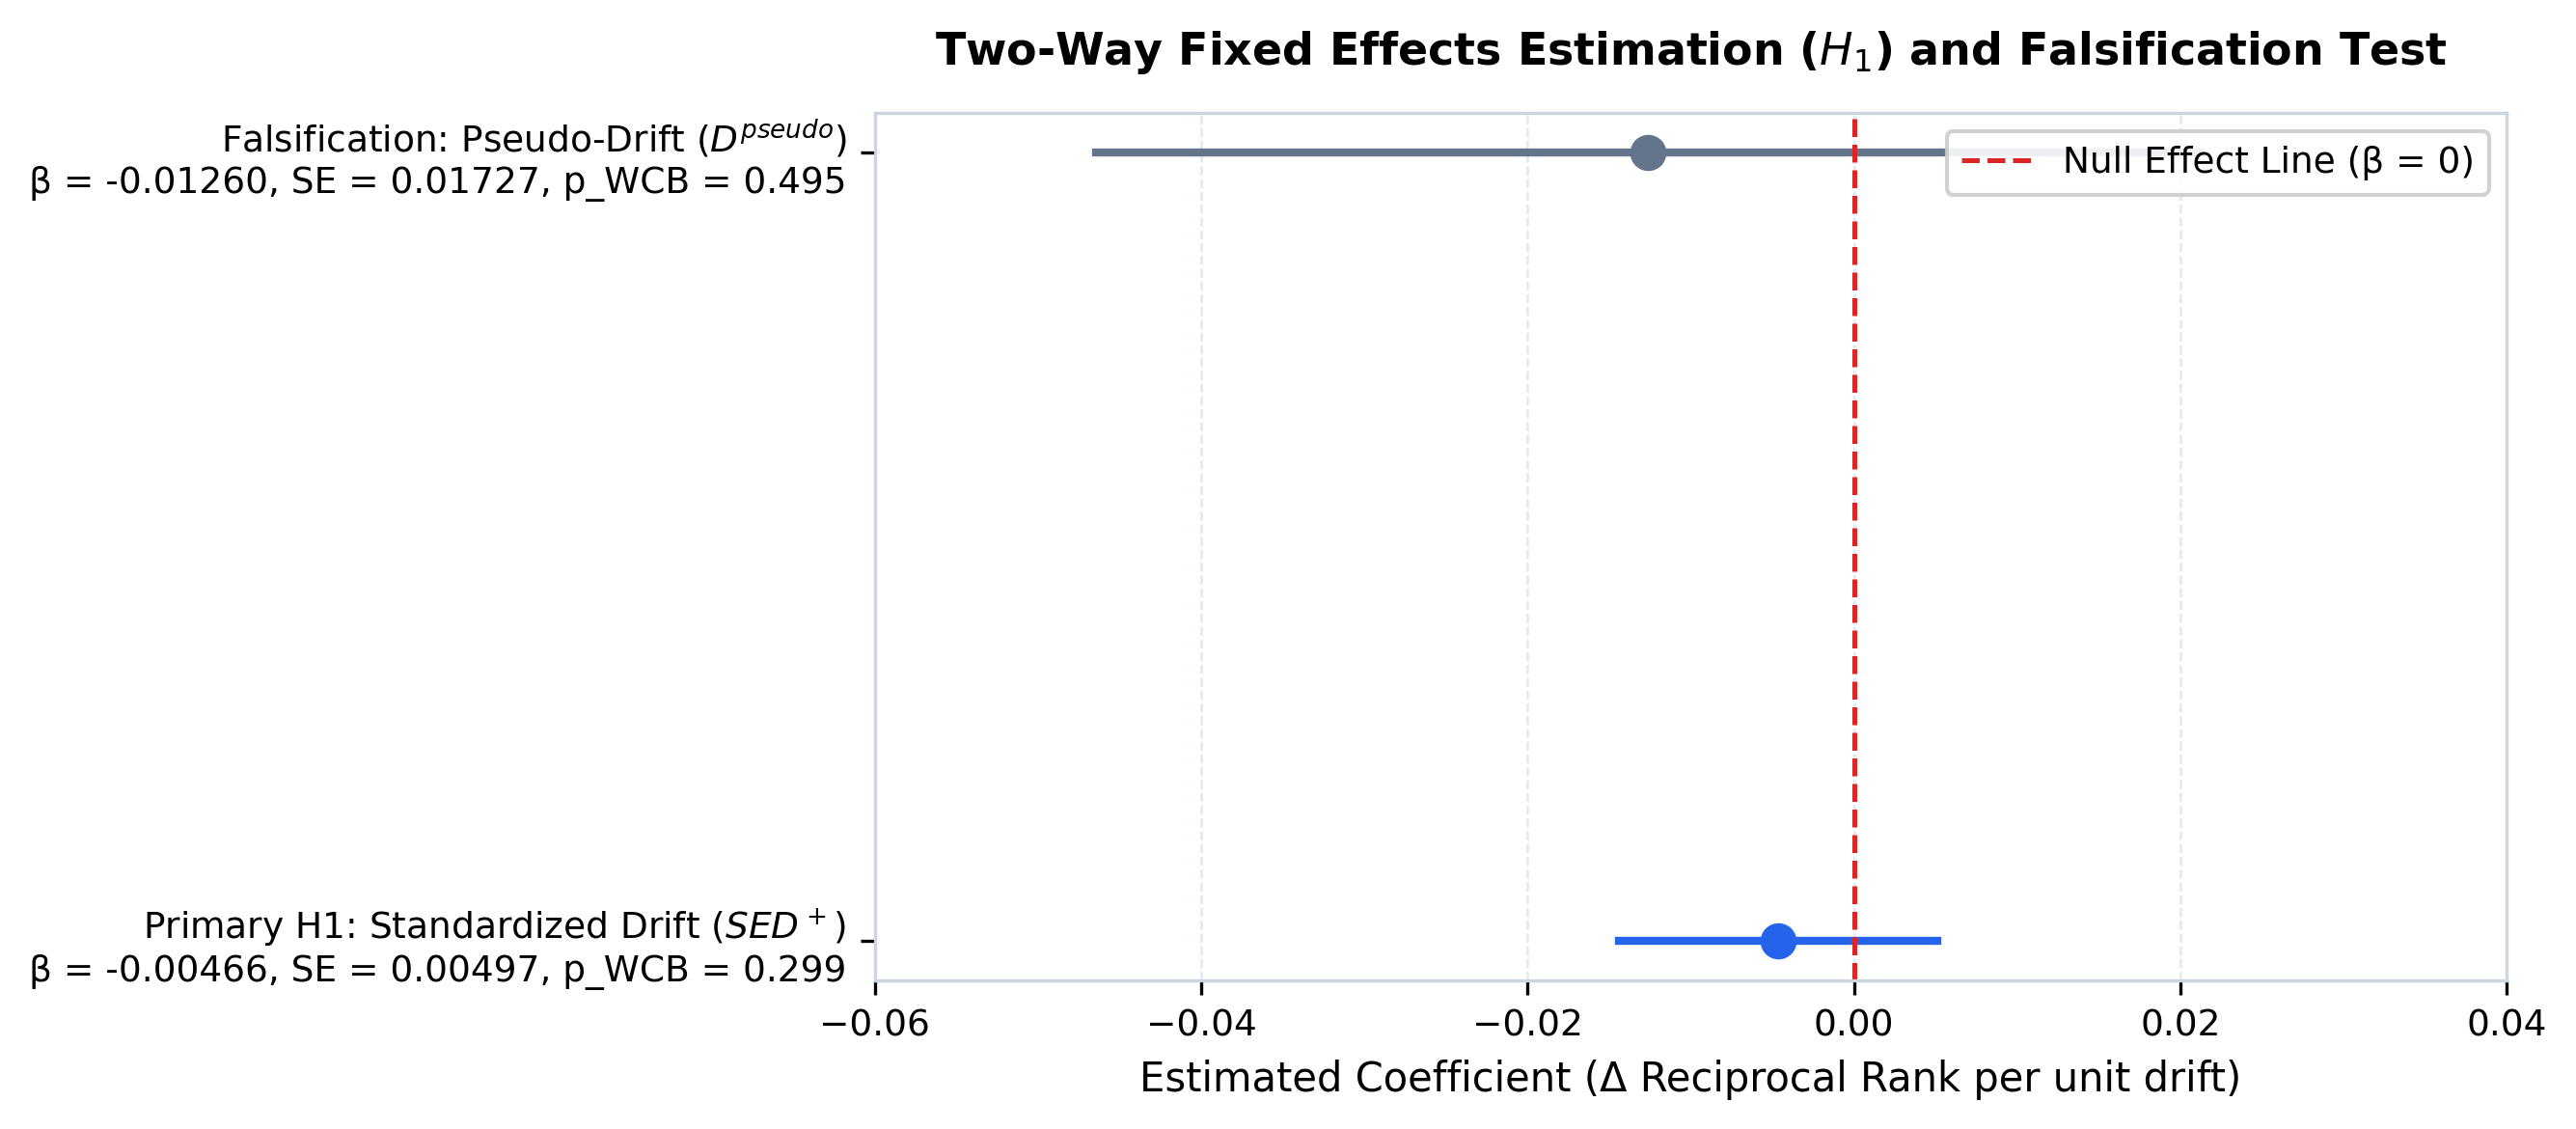
\includegraphics[width=0.85\textwidth]{figures/fig3_m4_twfe_h1_falsification_forest_plot.png}
\caption{Hình 3: Biểu đồ Forest Plot ước lượng hệ số tác động trôi dạt ($\beta_d$) và hệ số nhiễu giả định ($\beta_{\text{pseudo}}$) kèm khoảng tin cậy $95\%$.}
\label{fig:forest_plot_twfe}
\end{figure}

Ba kết luận khoa học cốt lõi rút ra từ Bảng~\ref{tab:twfe_econometric_results} và Hình~\ref{fig:forest_plot_twfe}:
\begin{enumerate}
    \item \textbf{Giả thuyết $H_1$ (Inconclusive):} Hệ số ước lượng mang dấu âm $\beta_d = -0.00366$ phù hợp với trực giác rằng trôi dạt biểu diễn làm giảm chất lượng suy luận. Tuy nhiên, với $SE = 0.00717$ và $p_{\text{WCB}} = 0.5740 > 0.05$, tác động này chưa đạt mức ý nghĩa thống kê $5\%$. Hệ thống kết luận trung thực là \textbf{INCONCLUSIVE}.
    \item \textbf{Kiểm định Phủ định Falsification (PASS):} Hệ số nhiễu thuần $\beta_{\text{pseudo}} = -0.01144$ với $p_{\text{WCB}} = 0.3810 \gg 0.05$. Điều này chứng minh quy trình đo lường không sinh ra tương quan giả tạo từ nhiễu ngẫu nhiên.
    \item \textbf{Phân tích Tương phản $H_2$:} Mức sụt giảm hiệu năng nội tại ($\Delta \text{MRR}_{\text{Seen-at-T1}} = -0.1384$) chiếm tới $83.7\%$ tổng mức sụt giảm trong thế giới mở ($-0.1654$), với khoảng lệch OOV bias gap đạt $-0.0270$.
\end{enumerate}
